%%%% Dokumentklassen %%%%

\documentclass[a4paper,11pt,fleqn,dvipsnames,twoside,openright]{memoir} 	% Openright åbner kapitler på højresider (openany begge)


%%%% PACKAGES %%%%

%% Oversættelse og tegnsætning %%
\usepackage[utf8]{inputenc}					% Input-indkodning af tegnsæt (UTF8)
\usepackage[danish]{babel}					% Dokumentets sprog
\usepackage[T1]{fontenc}					    % Output-indkodning af tegnsæt (T1)
\usepackage{ragged2e,anyfontsize}			% Justering af elementer
\usepackage{fixltx2e}						% Retter forskellige fejl i LaTeX-kernen
																			
%% Figurer og tabeller (floats) %%
\usepackage{graphicx} 						% Håndtering af eksterne billeder (JPG, PNG, EPS, PDF)
\usepackage{multicol}         	            	% Muliggør output i spalter
\usepackage{rotating}						% Rotation af tekst med \begin{sideways}...\end{sideways}
\usepackage{xcolor}							% Definer farver med \definecolor. Se mere: http://en.wikibooks.org/wiki/LaTeX/Colors
\usepackage{flafter}						% Sørger for at floats ikke optræder i teksten før deres reference
\let\newfloat\relax 						% Justering mellem float-pakken og memoir
\usepackage{float}							% Muliggør eksakt placering af floats, f.eks. \begin{figure}[H]

%% Matematik mm. %%
\usepackage{amsmath,amssymb,stmaryrd} 		% Avancerede matematik-udvidelser
\usepackage{mathtools}						% Andre matematik- og tegnudvidelser
\usepackage{textcomp}                 		% Symbol-udvidelser (fx promille-tegn med \textperthousand)
\usepackage{rsphrase}						% Kemi-pakke til RS-saetninger, fx \rsphrase{R1}
\usepackage[version=3]{mhchem} 				% Kemi-pakke til flot og let notation af formler, f.eks. \ce{Fe2O3}
\usepackage{siunitx}						% Flot og konsistent præsentation af tal og enheder med \si{enhed} og \SI{tal}{enhed}
\sisetup{output-decimal-marker = {,}}		% Opsætning af \SI (DE for komma som decimalseparator) 

%% Referencer og kilder %%
\usepackage[danish]{varioref}				% Muliggør bl.a. krydshenvisninger med sidetal (\vref)
\usepackage{natbib}							% Udvidelse med naturvidenskabelige citationsmodeller
\usepackage{xr}							    % Referencer til eksternt dokument med \externaldocument{<NAVN>}

%% Misc. %%
\usepackage{listings}						% Placer kildekode i dokumentet med \begin{lstlisting}...\end{lstlisting}
\usepackage{lipsum}							% Dummy text \lipsum[..]
\usepackage[shortlabels]{enumitem}			% Muliggør enkelt konfiguration af lister
\usepackage{pdfpages}						% Gør det muligt at inkludere pdf-dokumenter med kommandoen \includepdf[pages={x-y}]{fil.pdf}	
\pdfoptionpdfminorversion=6					% Muliggør inkludering af pdf-dokumenter, af version 1.6 og højere
\pretolerance=2500 							% Justering af afstand mellem ord (højt tal, mindre orddeling og mere luft mellem ord)	


%%%% CUSTOM SETTINGS %%%%

%% Marginer %%
\setlrmarginsandblock{3.5cm}{2.5cm}{*}		% \setlrmarginsandblock{Indbinding}{Kant}{Ratio}
\setulmarginsandblock{2.5cm}{3.0cm}{*}		% \setulmarginsandblock{Top}{Bund}{Ratio}
\checkandfixthelayout 						% Oversætter værdier til brug for andre pakker

%% Afsnitsformatering %%
\setlength{\parindent}{0mm}           		% Størrelse af indryk
\setlength{\parskip}{3mm}          			% Afstand mellem afsnit ved brug af double Enter
\linespread{1,1}							% Linjeafstand

%% Indholdsfortegnelse %%
\setsecnumdepth{subsection}		 			% Dybden af nummererede overskrifter (part/chapter/section/subsection)
\maxsecnumdepth{subsection}					% Dokumentklassens grænse for nummereringsdybde
\settocdepth{subsection} 					% Dybden af indholdsfortegnelsen
		
%% Opsætning af listings %%
\definecolor{commentGreen}{RGB}{34,139,24}
\definecolor{stringPurple}{RGB}{208,76,239}

\lstset{language=Matlab,					    % Sprog
	basicstyle=\ttfamily\scriptsize,		    % Opsætning af teksten
	keywords={for,if,while,else,elseif,		% Nøgleord at fremhæve
			  end,break,return,case,
			  switch,function},
	keywordstyle=\color{blue},				% Opsætning af nøgleord
	commentstyle=\color{commentGreen},		% Opsætning af kommentarer
	stringstyle=\color{stringPurple},		% Opsætning af strenge
	showstringspaces=false,					% Mellemrum i strenge enten vist eller blanke
	numbers=left, numberstyle=\tiny,		    % Linjenumre
	extendedchars=true, 					    % Tillader specielle karakterer
	columns=flexible,						% Kolonnejustering
	breaklines, breakatwhitespace=true,		% Bryd lange linjer
}

%% Navngivning %%
\addto\captionsdanish{
	\renewcommand\appendixname{Appendiks}
	\renewcommand\contentsname{Indholdsfortegnelse}	
	\renewcommand\appendixpagename{Appendiks}
	\renewcommand\appendixtocname{Appendiks}
	\renewcommand\cftchaptername{\chaptername~}		% Skriver "Kapitel" foran kapitlerne i indholdsfortegnelsen
	\renewcommand\cftappendixname{\appendixname~}	% Skriver "Appendiks" foran appendiks i indholdsfortegnelsen
}

%% Kapiteludssende %%
\definecolor{numbercolor}{gray}{0.7}		            % Definerer en farve til brug til kapiteludseende
\newif\ifchapternonum

\makechapterstyle{jenor}{					        % Definerer kapiteludseende frem til ...
  \renewcommand\beforechapskip{0pt}
  \renewcommand\printchaptername{}
  \renewcommand\printchapternum{}
  \renewcommand\printchapternonum{\chapternonumtrue}
  \renewcommand\chaptitlefont{\fontfamily{pbk}\fontseries{db}\fontshape{n}\fontsize{25}{35}\selectfont\raggedleft}
  \renewcommand\chapnumfont{\fontfamily{pbk}\fontseries{m}\fontshape{n}\fontsize{1in}{0in}\selectfont\color{numbercolor}}
  \renewcommand\printchaptertitle[1]{%
    \noindent
    \ifchapternonum
    \begin{tabularx}{\textwidth}{X}
    {\let\\\newline\chaptitlefont ##1\par} 
    \end{tabularx}
    \par\vskip-2.5mm\hrule
    \else
    \begin{tabularx}{\textwidth}{Xl}
    {\parbox[b]{\linewidth}{\chaptitlefont ##1}} & \raisebox{-15pt}{\chapnumfont \thechapter}
    \end{tabularx}
    \par\vskip2mm\hrule
    \fi
  }
}											        % ... her

\chapterstyle{jenor}						        % Valg af kapiteludseende - Google 'memoir chapter styles' for alternativer

%% Sidehoved %%

\makepagestyle{AAU}							        % Definerer sidehoved og sidefod udseende frem til ...
\makepsmarks{AAU}{%
	\createmark{chapter}{left}{shownumber}{}{. \ }
	\createmark{section}{right}{shownumber}{}{. \ }
	\createplainmark{toc}{both}{\contentsname}
	\createplainmark{lof}{both}{\listfigurename}
	\createplainmark{lot}{both}{\listtablename}
	\createplainmark{bib}{both}{\bibname}
	\createplainmark{index}{both}{\indexname}
	\createplainmark{glossary}{both}{\glossaryname}
}
\nouppercaseheads									% Ingen Caps ønskes

\makeevenhead{AAU}{\small ST2PRJ2 Gruppe 1}{}{\leftmark}	% Definerer lige siders sidehoved (\makeevenhead{Navn}{Venstre}{Center}{Hoejre})
\makeoddhead{AAU}{\rightmark}{}{\small ASE}		            % Definerer ulige siders sidehoved (\makeoddhead{Navn}{Venstre}{Center}{Højre})
\makeevenfoot{AAU}{\small \thepage}{}{}						% Definerer lige siders sidefod (\makeevenfoot{Navn}{Venstre}{Center}{Højre})
\makeoddfoot{AAU}{}{}{\small \thepage}						% Definerer ulige siders sidefod (\makeoddfoot{Navn}{Venstre}{Center}{Højre})

\copypagestyle{AAUchap}{AAU}							% Sidehoved for kapitelsider defineres som standardsider, men med blank sidehoved
\makeoddhead{AAUchap}{}{}{}
\makeevenhead{AAUchap}{}{}{}
\makeheadrule{AAUchap}{\textwidth}{0pt}
\aliaspagestyle{chapter}{AAUchap}					% Den ny style vælges til at gælde for chapters
													% ... her
															
\pagestyle{AAU}										% Valg af sidehoved og sidefod


%%%% CUSTOM COMMANDS %%%%

%% Billede hack %%
\newcommand{\figur}[4]{
		\begin{figure}[H] \centering
			\includegraphics[width=#1\textwidth]{billeder/#2}
			\caption{#3}\label{#4}
		\end{figure} 
}

%% Specielle tegn %%
\newcommand{\decC}{^{\circ}\text{C}}
\newcommand{\dec}{^{\circ}}
\newcommand{\m}{\cdot}


%%%% ORDDELING %%%%

\hyphenation{}


%%%% Tilføjelser af min preample %%%%

% Booktabs:
% The booktabs package is needed for better looking tables. 
\usepackage{booktabs}

% Caption:
% For better looking captions. See caption documentation on how to change the format of the captions.
\usepackage[hang, font={small, it}]{caption}

% Hyperref:
% This package makes all references within your document clickable. By default, these references will become boxed and colored. This is turned back to normal with the \hypersetup command below.
\usepackage{hyperref}
	\hypersetup{colorlinks=false,pdfborder=0 0 0}

% Cleveref:
% This package automatically detects the type of reference (equation, table, etc.) when the \cref{} command is used. It then adds a word in front of the reference, i.e. Fig. in front of a reference to a figure. With the \crefname{}{}{} command, these words may be changed.
\usepackage{cleveref}
	\crefname{equation}{formel}{formler}
	\crefname{figure}{figur}{figurer}	
	\crefname{table}{tabel}{tabeller}

% Mine tilføjelser:
\usepackage{units}                        %% Bruges til at gøre fx 1/2 samlet med: \nicefrac{1}{2}.
\usepackage{tabu, longtable}              %% Bruges til tabeller.
\setlength{\tabulinesep}{1.5ex}           %% Definerer linjeafstand i tabeller.
\usepackage{enumerate}                    %% Bruges til lister.
\usepackage{tabto}                        %% Giver mulighed for TAB med fx \tabto{3em}.
\usepackage[hyphenbreaks]{breakurl}       %% Bruges til websiders url'er.
\renewcommand{\UrlFont}{                  %% Definerer url-font.
\small\ttfamily}                          %
\bibliographystyle{plain}                 %% Definere bibliografien. Ses til sidst i dokumentet i kapitlet Litteratur.
\raggedbottom

%\externaldocument[D-]{Dokumentation}

\begin{document}	
\frontmatter						% Nummereres med romerske tal.
\begin{titlingpage}
\begin{center}

~ \\[3cm]


\includegraphics[width=0.6\textwidth]{figurer/ASE.png}~\\[1cm]

\textsc{\LARGE Aarhus School of Engineering}\\[1.5cm]

\textsc{\Large Sundhedsteknologi}\\
\textsc{\Large 2. semesterprojekt}\\[0.5cm]

\noindent\makebox[\linewidth]{\rule{\textwidth}{0.4pt}}\\
[0.5cm]{\Huge Rapport}
\noindent\makebox[\linewidth]{\rule{\textwidth}{0.4pt}}

\end{center}

\textit{Gruppe 1} \newline
Lise Skytte Brodersen (201407432) \newline
Mads Fryland J\o rgensen (201403827) \newline
Albert Jakob Fredshavn (201480425) \newline
Malene Cecilie Mikkelsen (201405722) \newline		 
Mohamed Hussein Mohamed (201370525) \newline 
Sara-Sofie Staub Kirkeby (201406211) \newline
Martin Banasik (201408398) \newline
Cecilie Ammizb\o ll Aar\o e (201208778) \newline 


\textit{Vejleder} \newline
Studentervejleder\\
Lars Mortensen\\
Aarhus Universitet\\
\pageref{LastPage}



\vfill

\begin{center}
{\large \today}
\end{center}


\end{titlingpage}
\chapter{Resumé}
\begin{vplace}[0.6]
{\large \textit{Gruppemedlemmer}}
\\
\\

\noindent \begin{tabular}{ll}
	\makebox[3.0in]{\hrulefill} & \makebox[1.5in]{\hrulefill}\\
	Lise Skytte Brodersen (201407432) & Dato\\[7ex]% adds space between the two sets of signatures
	\makebox[3in]{\hrulefill} & \makebox[1.5in]{\hrulefill}\\
	Mads Fryland J\o rgersen (201403827) & Dato\\[7ex]
	\makebox[3in]{\hrulefill} & \makebox[1.5in]{\hrulefill}\\
	Albert Jakob Fredshavn (201408425) & Dato\\[7ex]
	\makebox[3in]{\hrulefill} & \makebox[1.5in]{\hrulefill}\\
	Malene Cecilie Mikkelsen (201405722) & Dato\\[7ex]
	\makebox[3in]{\hrulefill} & \makebox[1.5in]{\hrulefill}\\
	Mohamed Hussein Mohamed (201370525) & Dato\\[7ex]
	\makebox[3in]{\hrulefill} & \makebox[1.5in]{\hrulefill}\\
	Sara-sofie Staub Kirkeby (201406211) & Dato\\[7ex]
	\makebox[3in]{\hrulefill} & \makebox[1.5in]{\hrulefill}\\
	Martin Banasik (201408398) & Dato\\[7ex]
	\makebox[3in]{\hrulefill} & \makebox[1.5in]{\hrulefill}\\
	Cecilie Ammitzb\o ll Aar\o e (201208778) & Dato\\[7ex]
	
\end{tabular}
\\
{\large \textit{Vejleder}}
\\
\\
\\
\noindent \begin{tabular}{ll}
	\makebox[3.0in]{\hrulefill} & \makebox[1.5in]{\hrulefill}\\
	Lars Mortensen & Dato\\[8ex]
\end{tabular}
\end{vplace}

\chapter{Godkendelsesformular}

{\LARGE\textit{Godkendelsesformular}}

{\large Forfattere:}
\\[5ex]


\begin{tabular}{c c}
\centering 
	\makebox[2.0in]{\hrulefill} & \makebox[2.0in]{\hrulefill}\\
	Lise Skytte Brodersen & Mads Fryland Jørgensen\\[7ex]
	\makebox[2.0in]{\hrulefill} & \makebox[2.0in]{\hrulefill}\\
	Albert Jakob Fredshavn & Malene Cecilie Mikkelsen\\[7ex]
	\makebox[2.0in]{\hrulefill} & \makebox[2.0in]{\hrulefill}\\
	Mohamed Hussein Mohamed & Sara-Sofie Staub Kirkeby\\[7ex]
	\makebox[2.0in]{\hrulefill} & \makebox[2.0in]{\hrulefill}\\
	Martin Banasik & Cecilie Ammitzøll Aarøe\\[7ex]

\end{tabular}

\begin{tabular}{c c c c}
	\textbf{Godkendes af:} & Lars Mortensen\\[3ex]
	\textbf{Antal sider} & <antalsider>\\[3ex]
	\textbf{Kunde} & Aarhus Universitet
\end{tabular}\\[8ex]
Ved underskrivelse af dette dokument accepteres det af begge parter som værende kravene til udviklingen af det ønskede system.
\\
\\
\textbf{Dato: } 28/5-2015\\[7ex]

\begin{tabular}{c c}
	\makebox[2.0in]{\hrulefill} & \makebox[2.0in]{\hrulefill}\\
	\centering 
	Kundens underskrift & Leverandørens underskrift
\end{tabular}

\chapter{Ordliste}

\begin{longtabu} to \linewidth{@{}l X[j]@{}}
    Ord &    Forklaring\\
    \toprule 
	EKG	&	Elektrokardiografi\\
	DAQ	&	Data acquisition\\
	AV-klapper	&	Atrioventrikulær-klapperne\\
	AV-knuden	&	Atrioventrikulær-knuden\\
	ISE & Indledende System Engineering \\
	SysML & System Modeling Language \\
	BDD & Block Defination Diagram \\
	IBD & Intern Block Diagram\\
	SD & Sekvensdiagram\\
	UML & Unified Modeling Language\\
	Cerebral apopleksiske &	Slagtilfælde i hjernen (blodprop/hjerneblødning)\\
	Hjerteinsufficiens	&	Hjertesvigt\\
\label{forkort}
\end{longtabu}
\cleardoublepage		

\tableofcontents*                   % Indsætter en indholdsfortegnelse før Indledning.

\mainmatter                         % Her findes de nummererede kapitler modsat \frontmatter og \backmatter. Nummereres med arabiske tal.
\subsubsection{Versionhistorik}

\begin{longtabu} to \linewidth{@{}l l l X[j]@{}}
    Version &    Dato &    Ansvarlig &    Beskrivelse\\[-1ex]
    \midrule
    Tekst &    Tekst &    Tekst &    Tekst.\\
\label{version_Systemark}
\end{longtabu}

\chapter{Indledning}
I dagens Danmark er incidensen af hjertesygdomme på ca. 45.000 nye tilfælde årligt\footnote{http://www.si-folkesundhed.dk/upload/hjertekarsygdomme\_i\_2011-2\_rapport.pdf}. Mange typer af hjertesygdomme diagnosticeres via et EKG-apparat, der måler patientens hjerteimpulser. Disse impulser bliver afbildet som en graf, der indeholder P-, Q-, R-, S- og T-takker. Det er forholdet mellem disse takker, der fortæller, hvordan hjerteimpulserne hos patienten er. Hvis en patient har et rask EKG-signal, skal forholdet mellem takkerne være indenfor nogle bestemte intervaller. Et EKG-signal, der afviger fra disse standarter siges at være abnormalt og patienten bør tjekkes for en eventuel hjertesygdom. Derfor er et EKG-apparat en vigtig teknologi indenfor sundhedsvæsenet i forhold til videre diagnosticering af hjertesygdomme.\\ \\
Formålet med dette projekt er, at udvikle en software, som netop har til formål at detektere en selvvalgt hjertesygdom. Den nødvendige hardware samt et stykke kode, der betragtes som Blackbox, er blevet udleveret ved projektets start.\\
Dette specifikke projekt omhandler sygdommen atrieflimren. En sygdom, der særligt omfatter den ældre befolkning, da prævalensen i Danmark er 5-10\%\footnote{https://www.sundhed.dk/borger/sygdomme-a-aa/hjerte-og-blodkar/sygdomme/hjertearytmier/atrieflimren-og-flagren/} for borgere over 80 år.\\
Atrieflimren forekommer, når patientens atrie-kontraktionsmønster forstyrres og dermed begynder at flimre. Atrieflimren karakteriseres ved, at der forekommer 220-300 små udsving pr. minut på EKG-signalets baseline. Desuden vil der i frekvensspektret 300-400 Hz, opstå forhøjede amplituder. Det er ud fra denne karakteristik af amplituder, der, i Visual Studio, er blevet udarbejdet en analyse, som kan detektere atrieflimren. Denne analyse er en del af et større program, hvis formål også er, at kunne visualisere og gemme et et givet EKG-signal i en privat- samt offentlig database. \\ \\
Rapporten er udført som en naturvidenskabelig rapport med først og fremmest et baggrundsafsnit. Dette afsnit fortæller overordnet omkring hjertets funktionalitet, atrieflimren og elektrokardiografi. Det er denne teori, som ligger til grund for systemets design og opbygning, samt hvilke krav, der er stillet til systemet.
  

\chapter{Projektformulering}
\section{Problemformulering}
 I dette projekt vil vi udvikle en software, som ud fra en virtuel patients EKG-målinger kan detektere atrieflimmer. 
\section{Indledning}
Via kendskabet til raske EGK-signaler, ved vi hvordan forholdet mellem P-, Q-, R-, S- og T-takkerne normalt er. Ud fra dette kan vi programmere et system, som kan analysere et givet abnormalt EKG-signal, og dermed informere brugeren fx i form af sundhedsfagligt personale om eventuelle forekomster af atrieflimmer.\\
Udover at detektere og informere om atrieflimmer kan softwaren også danne en graf og gemme de givne data i en SQL-database. Softwaren er opbygget via trelagsmodellen, som består af et data-, logik- og GUI-lag.
\\
Det abnormale EKG-signal hentes ned i form af en csv-fil fra den eksterne EKG-database, Physionet (lav reference eller ordliste). Csv-filens data omdannes via Analog-discovery til et analogt signal. Det analoge signal omdannes via DAQ'en til et digitalt signal. Det er dette digitale signal softwaren behandler, og er dermed det signal, der dannes en graf ud fra. Softwaren detekterer atrieflimmer og informerer brugeren herom.     


1. rask hjerte\\
2. EKG-signaler generelt inkl. beskrivelse af takker\\
3. patofysiologi - atrieflimmer inkl. detektion via EKG\\
4. Software og hardware beskrivelse
\chapter{Baggrund}

\section{Hjertet}
Hjertet, \textit{cor}, er en hul muskel, der har til opgave at pumpe blodet rundt til hele kroppen. Hjertet består af i alt fire kamre, som det kan ses på figur 3.1 nedenfor. To forkamre, atrier, og to hjertekamre, ventrikler. Atrierne fungere primært som reservoir for blod, mens ventriklerne fungerer som den effektive pumpe.\\

\begin{figure}[htb]
	\centering
	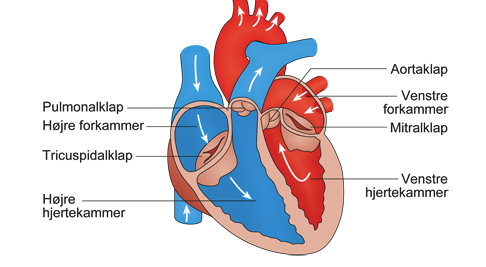
\includegraphics[width=1\textwidth]{Figurer/Snip20150410_31}
	\caption{Hjerte med forklarende pile \protect\footnotemark} 
\end{figure}
\footnotetext{http://www.hjertelunge.dk/hjertesygdomme/hjerte\_og\_kredsloeb/hjertet/}

Hjertekamrene og forkamrene er adskilt fra hinanden af anulus fibrosus, som er en plade af bindevæv. Anulus fibrosus består af fire bindevævsringe, der er forbundet med hinanden. To af disse udgør åbningerne mellem atrierne og ventriklerne. De to sidste danner åbningerne mellem højre hjertekammer og lungepulsåren og venstre ventrikel og hovedpulsåren. Ved alle bindevævsringene er der klapper, der fungere som ventiler.\\ 
AV-klapperne sidder mellem atrierne og ventriklerne. Klappen mellem højre atrium og ventrikel kaldes tricuspidalklap, mens klappen mellem venstre atrium og ventrikel kaldes mitralklap, se figur 3.1. Aortaklappen er placeret ved afgangen af hovedpulsåren og pulmonalklappen ved afgangen af lungepulsåren. Klapperne fungere således, at blodet kun kan løbe én vej gennem dem. Åbningen samt lukningen af disse er en passiv proces, som bestemmes af forskelle i væsketrykket på de to sider af klapperne.\\ 

\begin{figure}[htb]
	\centering
	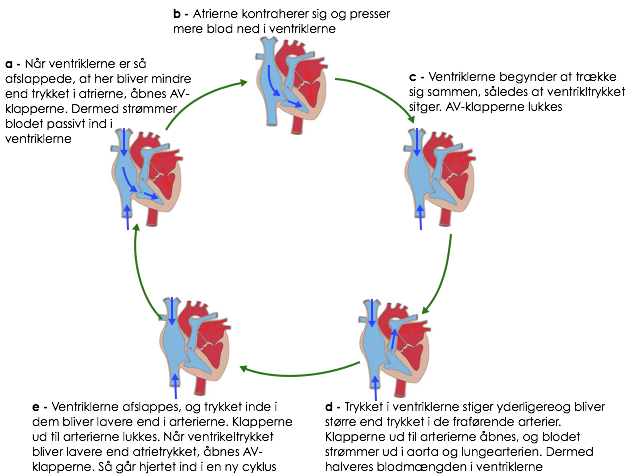
\includegraphics[width=1\textwidth]{Figurer/Snip20150412_7}
	\caption{De forskellige faser i hjertets cyklus \protect\footnotemark}
\end{figure}
\footnotetext{Billede fra "Menneskets anatomi og fysiologi" s. 273 figur 9.6}

Hjertets cyklus, som er illustreret ved figur 3.2, inddeles i to hovedfaser. Den første kaldes diastolen. I diastolen er ventriklerne afslappede og fyldes med blod. Det vil sige, at trykket i ventriklerne bliver lavere end trykket i atrierne, således at AV-klapperne åbnes, og blodet begynder at strømme ind i ventriklerne. Under hele diastolen er aortaklappen lukket. Den anden fase kaldes systolen. I systolen kontraherer ventriklerne sig. Trykket i ventriklerne overstiger trykket i atrierne således, at AV-klapperne lukkes, så tilbagestrømning af blod til atrierne forhindres. Når ventriklerne har kontraheret sig så meget, at trykket i ventriklerne overstiger trykket i hovedpulsåren samt i lungepulsåren, åbnes aortaklappen og pulmonalklappen, og blodet strømmer ud i hovedpulsåren og lungepulsåren. Ventriklernes tryk falder igen til under atriernes tryk, hvilket påvirker, at AV-klapperne åbnes igen og hjertets cyklus starter forfra.\\
Hjertets cyklus igangsættes i sinusknuden ved aktionspotentialer, der føres til de forskellige dele af hjertet. Dette sker enten ved, at aktionspotentialet går fra hjertemuskelcelle til hjertemuskelcelle gennem åbne celleforbindelser, eller gennem åbne celleforbindelser mellem specialiserede hjertemuskelceller i hjertets specielle ledningssystem. Det specielle ledningssystem består af tre sammenhængende dele - AV-knuden, det hiske bundt gennem anulus fibrosus og det hiske bundt over i purkinjefibrene(se figur 3.3). \\
Hjertets ledningssystem har to hovedopgaver. Først at sørge for, at aktionspotentialet spredes hurtigt gennem hjertet, og dermed sørge for al hjertemuskulaturen i ventriklen kontraheres næsten samtidig. Denne næsten samtidige kontraktion medfører, at der inde i ventriklerne opbygges et effektivt tryk. Purkinjefibrene, som kun er i ventriklerne og ikke atrierne, gør at aktionspotentialerne spredes hurtigere i ventriklerne end i atrierne. Den anden hovedopgave er derfor at sikre en vis forsinkelse i impulsledning fra atrierne til ventriklerne. Forsinkelsen er mulig, da anulus fibrosus fungerer som en elektrisk isolator. Derfor skal aktionspotentialet ledes fra atrierne til ventriklerne via det specialiserede ledningssystem, og da AV-knuden leder aktionspotentialet særlig langsomt, opstår forsinkelsen. Dette medfører, at atriernes kontraktion fuldføres, før ventriklernes igangsættes, dermed er der sikret en tilstrækkelig fyldning af ventriklerne, før de pumper blodet videre. Denne spredning og udløsning af aktionspotentiale sker regelmæssigt, og er den afgørende faktor for hjertets kontraktions rytme.
\begin{figure}[htb]

	\centering	
	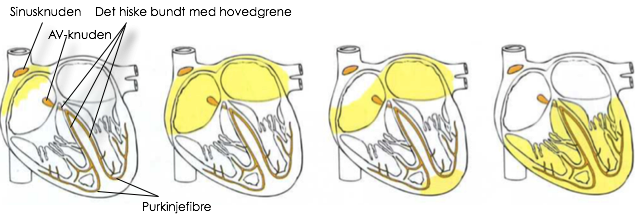
\includegraphics[width=1\textwidth]{Figurer/Snip20150410_6}
	\caption{Spredning af aktionspotentialer gennem hjertet \protect\footnotemark}
\end{figure}
\footnotetext{"Menneskets anatomi og fysiologi" s. 275 figur 9.9}

I figur 3.3 ses spredningen af aktionspotentialer gennem hjertet. Aktionspotentialet udløses i sinusknuden og forsinkes i AV-knuden. Dernæst ledes aktionspotentialet videre til ventrikelmuskulaturen. De farvelagte områder er de depolariserede områder og det ses, at atriernes depolarisering er afsluttet før ventriklernes er startet.

\section{Elektrokardiogram}
Et elektrokardiogram, EKG, afspejler hjertets elektriske aktivitet. Teknikken kaldes elektrokardiografi og udføres via elektroder, der er placeret forskellige steder på kroppen, primært omkring hjertet. Elektroderne måler den elektriske aktivitet via en overfladespænding, der går ud fra thorax. Det er disse elektriske spændinger, som danner de forskellige graf-udsving, som er EKG-signalets takker. Takkerne viser atriernes- og ventriklernes systole og diastole, og er inddelt i P-takken, QRS-komplekset og T-takken. Grafisk vil EKG signalet være vist som det ses på figur 3.4 nedenfor.

\begin{figure}[H]
	\centering
	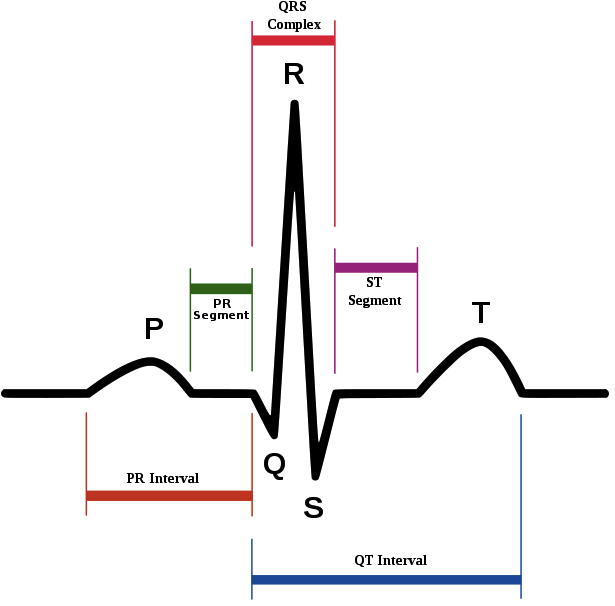
\includegraphics[width=0.7\textwidth]{Figurer/Snip20150412_36}
	\caption{Normalt EKG-signal \protect\footnotemark}
\end{figure}
\footnotetext{http://en.wikipedia.org/wiki/QRS\_complex\#/media/File:SinusRhythmLabels.svg}

P-takken viser atriets depolarisering. Dernæst kommer PR-segmentet, som er den forsinkede strøm fra atrier til ventrikler. QRS-komplekset udgør ventrikeldepolariseringen. QRS-komplekset er større end P-takken, da muskelmassen i ventriklerne er større end atriernes muskelmasse, hvilket påvirker en højere elektrisk aktivitet. T-takken beskriver ventriklernes repolarisering. Denne er også mindre end QRS-komplekset, da repolariseringen forløber langsommere end depolariseringen.\\
Elektrokardiografi giver et billede af, hvordan hjertet fungerer. På figur 3.4 ses et EKG-signal for et raskt hjerte. Ved et raskt hjerte vil intervallerne mellem takkerne i EKG-signalet være følgende: 

\begin{itemize}
	\item PR Interval: 0.12 - 0.20 sekunder
	\item QRS Complex: 0.08 - 0.10 sekunder 
	\item QT Interval: 0.4 - 0.43 sekunder 
	\item RR Interval: 0.6 - 1.0 sekunder 
\end{itemize}

 Hvis hjertet ikke fungere optimalt, vil EKG-signalet se anderledes ud, og en sundhedsfaglig person vil kunne diagnosticere eventuelle sygdomme ud fra grafen.  En patient kunne eventuelt have atrieflimren, som er den sygdom, dette projekt omhandler.  


\section{Atrieflimren}
Atrieflimren forekommer, når atrierne ikke kontraherer sig ordentligt. Den hyppigste udløsning af atrieflimren forefalder pga. en serie af hurtige impulser (ekstrasystoler), hvilket er illustreret på første del af figur 3.5.  Ekstrasystolerne kommer fra den atriemuskulatur, som sidder nær lungevenerne i venstre atrium. Dermed bliver atriernes normale kontraktionsmønster ødelagt, og de begynder at "flimre". Under atrieflimren fungerer sinusknuden stadig som normalt, men har ingen kontakt til atrium.\\
Pga. arytmien mister man den regelmæssige atrietømning og får nedsat funktion af hjertets pumpning. Blodet vil ophobe sig i atriet og danne lokale tromber.  De kan løsrive sig og flyde med blodstrømmen ud i kroppen, hvor de kan sætte sig fast (embolisere). Ubehandlet emboliserende atrieflimren er årsagen til 1/3 af alle cerebral apopleksiske tilfælde. Derfor er det vigtigt at være opmærksom på tilstedeværelse af atrieflimren hos netop disse patienter.\\
Hvis arytmien står på i længere tid, og ventrikelfrekvensen er hurtig, kan det udløse hjerteinsufficiens med tiltagende dilatation og dårlig kontraktion af ventriklerne. \\
Atrieflimren opstår som anfald (paroksystisk), der spontant konverterer tilbage til normal sinusrytme efter få timer til dage. Med årerne bliver arytmien mere vedvarende (persisterende) for til sidst at blive kronisk.  De symptomer, som kan forbindes med atrieflimren er en øget træthed, åndenød og en forhøjet samt uregelmæssig puls, der kan være utydelig og hurtig. Desuden vil blodtrykket falde, og der kan være tegn på hjerteinsufficiens, både i højre og venstre side af hjertet. 

\begin{figure}[htb]
	\centering
	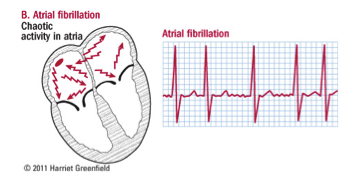
\includegraphics[width=1\textwidth]{Figurer/Snip20150412_32}
	\caption{Aktivitet i atrie ved atrieflimren\protect\footnotemark}
\end{figure}
\footnotetext{http://www.health.harvard.edu/heart-health/atrial-fibrillation-common-serious-treatable}

Diagnosen stilles via elektrokardiografi. EKG-grafen er domineret af mange irregulære og smalle QRS-komplekser uden ordentlige P-takker, som set på figur 3.5 ovenover. Med andre ord siges det, at der forekommer 220-300 små udsving/minut. Der kan også være forhøjede amplituder i frekvensspektret 300-400 Hz. Hvis disse forhold forekommer, kan patienten muligvis have atrieflimren.\\ 
Den hyppigste form for behandling er ved betablokkere, flekainid, dronaderon og amiodaron. Der indføres katere i venstre atrium, som ødelægger atriemuskulaturen, hvilket udløser flimren.

  
\chapter{Systembeskrivelse}

Overordnet set, består systemet af en hardware- og en software-del.\\ Hardwaren er blevet udleveret og består af en DAQ og Analog-discovery. DAQ'en og Analog-discovery har begge forbindelse til computeren, som har forbindelse til hinanden. Se figur 4.1.  

\begin{figure}[H]
	\centering
	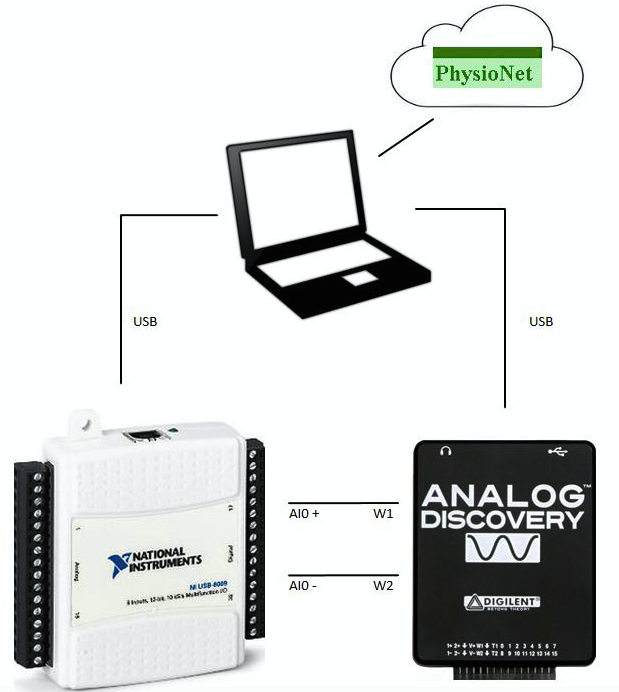
\includegraphics[width=0.45\textwidth]{Figurer/Snip20150427_1}
	\caption{Opstilling af Hardwaren}
\end{figure}

I projektet analyseres virtuelle patienters EKG-signaler. Disse EKG-signaler kommer fra PhysioNet, som er ekstern database, der kan tilgås via internettet\footnote{www.physionet.org}. EKG-signalet, der ønskes analyseret, hentes ned som en CSV-fil. Filens information bliver omdannet til et analogt signal, som simuleres af Analog-discovery. Det analoge signal bliver konverteret til et digitalt signal af DAQ'en. Det er dette digitale signal, som systemet kan afbilde og analysere.
\\ \\
Softwaren for systemet er kernen i dette projekt. Der er blevet udleveret et program, der anses som en blackbox. Dette program skabes der reference til således, at systemet kan fungere optimalt. Softwaren kan illustrere og analysere EKG-signaler med henblik på atrieflimren. Systemet kan desuden lagre information om signalerne i en privat- og offentlig database.\\
Projektets endelige produkt er en prototype af et software system, som kan benyttes i et EKG-apparat.            


\chapter{Krav}
\chapter{Projektbeskrivelse}

\section{Projektgennemførelse}
Projektet startede med, at der blev lavet en tidsplan, som var mulig at ændre undervejs, dog med faste deadlines, som skulle overholdes. De forskellige deadlines lagde op til, at der kunne arbejdes efter vandfaldsmodellen, hvilket dette projekt følger, se figur 6.1. Vandfaldsmodellen går ud på, at der først stilles nogle krav til produktet. Derefter designes produktet på papiret, hvor udseende og kunnen beskrives. Efterfølgende implementeres produktet ud fra krav og design. Til slut udføres en accepttest, hvor der testes i forhold til de funktionelle og ikke-funktionelle krav, der er stillet til produktet.

\begin{figure}[H]
	\centering
	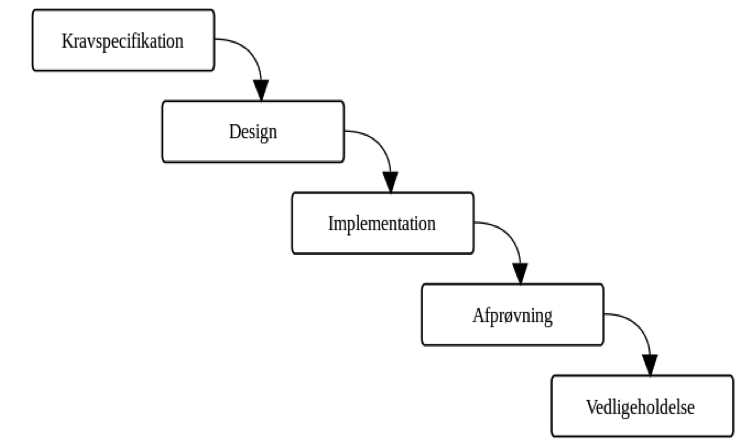
\includegraphics[width=1\textwidth]{Figurer/Snip20150522_15}
	\caption{Vandfaldsmodel}
\end{figure}

Projektgruppen har været på 8 medlemmer, som er blevet delt ind i 2 grupper. Den ene gruppe arbejdede med softwareudviklingen, mens den anden gruppe arbejdede med dokumentation og udarbejdelsen af design. Da gruppen har været opdelt, har der været projektmøde hver uge, hvor gruppen har opdateret hinanden og rettet tidsplanen til, hvis det var nødvendigt.


\section{Metode} 
Dette afsnit har til formål at beskrive hvilke metoder, der er benyttet i udarbejdelsen af projektet. Primært er der tale om metoder fra faget ISE samt Sundhedsvidenskab.\\ 
Desuden bliver der i dette afsnit også beskrevet hvilke arbejdsredskaber, der er benyttet til udførelse af projektet, rapporten og dokumentationen.\\ \\
Til beskrivelse samt opbygning af EKG-systemet er der fra ISE benyttet metoden SysML. SysML er en metode, der vha. digrammer analyserer, specificerer, designer og verificerer et givet system. Altså er metoden benyttet til at beskrive systemets opbygning og kommunikationen. \\ 
Yderligere er der en applikationsmodel, som giver samlet overblik over systemet. Denne model består af en domænemodel, hvor alle aktiviteterne i systemet er beskrevet samt tilhørende klassediagrammer med metoder fra sekvensdiagrammer. SD beskriver systemets virkning, og hvordan de enkelte dele interagerer, hvilket er specifikt for hver enkelt use case.\\ 
Softwaren er beskrevet gennem metoden UML, helt specifikt ved et UML klassediagram. Klassediagrammet viser, hvilke klasser og metoder al softwaren (med undtagelse af blackbox) består af, samt hvordan systemet er bygget op efter trelagsmodellen.\\
Baggrundsafsnittet, afsnit 3, er udarbejdet ved tekstanalyse og kildekritik, ud fra sundhedsvidenskabelige bøger.\\ \\
Af benyttede arbejdsredskaber er der først og fremmest brugt en fælles arbejdsplatform, GitHub. GitHub er en online platform, hvor der er mulighed for at foretage ændringer samtidigt, og gemme i en fælles mappe. Yderligere er der mulighed for en detaljeret versionshistorik.\\
Alle SysML- og UML-diagrammer er udarbejdet i programmet Visio. Koden er skrevet i sproget C\# i programmet Visual Studio. Visual Studio spiller også sammen med programmet WaveForms Generator, i forbindelse med simulering af EKG-signalet. Selve rapporten, mødereferater, logbog og dokumentationen er udformet i tekstprogrammet LaTex. Yderligere er Facebook brugt til mødeindkaldelse og generel kommunikation.



\section{Specifikation og analyse}

I udarbejdelsen af analysen var der mange komplikationer. Dette skyldes primært, at atrieflimren ikke nødvendigvis påvirker et EKG-signal på samme måde hver gang.\\ \\
Først var der tiltænkt en analyse, som skulle tage udgangspunkt i definition for atrieflimren, hvor der forekommer 220-300 små udsving/minut på baselinen. Baseline er et udtryk for den linje, som svingningerne centrerer sig omkring. Måden hvorpå dette skulle foregå, var ved at tage et gennemsnit af baselinens støj, altså de stykker af EKG-signalet, som ikke udgør P-, Q-, R,- S, og T-takkerne. Derefter detekteres hvor mange gange der skete en svingning over baselinen. Her skulle der så tjekkes, om svingningerne overtrådte en tærskel. Denne tærskel skulle vurderes ud fra den patofysiologiske baggrund for sygdommen. Efter visualisering af reelle målinger, blev denne metode dog afskrevet, da baseline ikke bliver repræsenteret ved en regulær linje i reelle signaler. \\ \\ 
Derefter blev der udtænkt en metode med en dynamisk baseline. Denne metode viste sig meget tidligt i udviklingsprocessen ikke at være kompatibel. Den største komplikation ved denne metode var at udarbejde en analyse, der kunne udelukke de kendte takker, som karakteriserer et EKG-signal. Hvis denne analyse ikke blev fundet, ville den dynamiske baseline altid ligge et stykke over den reelle baseline, grundet de høje R-takker. \\ \\
De to første metoder blev aldrig færdiggjort, da problemerne opstod efter pseudokoden blev udarbejdet. Herefter gik gruppen til vejleder for at finde en alternativ løsning til analysen. Vejleder fik herefter input fra en anden professionel, og kunne derefter hjælpe med at udarbejde en analyse, som virkede.\\
Vejleder kunne oplyse, at atrieflimren har specifikke kendetegn, hvis der bliver analyseret på EKG-signalets amplituder inden for specifikke frekvenser. Det er ud fra denne information, at den endelige analyse blev udarbejdet. 

\section{Arkitektur}
Softwaren er bygget op i henhold til trelagsmodellen, hvor GUI’erne fungerer som programmets brugerinterface, med et login-vindue, et CPR-vindue og et EKG-vindue. Her fungerer EKG-vinduet, som det primære vindue, hvor EKG-signaler kan vises, analyseres og gemmes. Præsentationslaget er yderligere beskrevet i dokumentationen 3.3.1, men kan også visualiseres ud fra figur 6.2 nedenfor.

\begin{figure}[H]
	\centering
	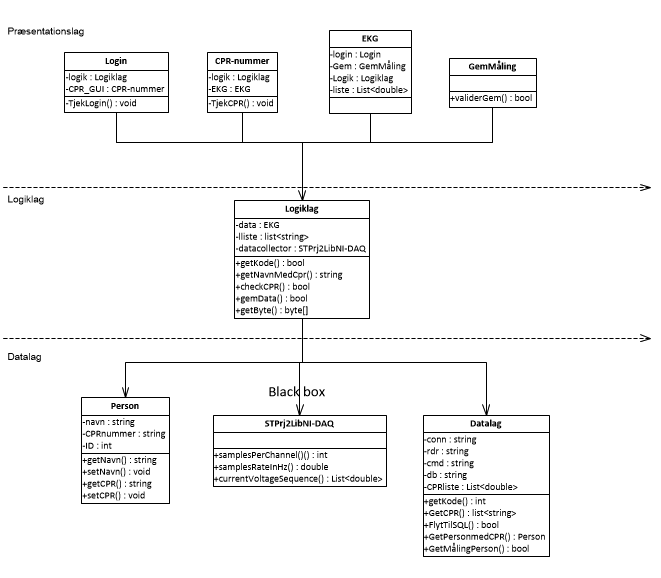
\includegraphics[width=0.9\textwidth]{Figurer/Snip20150527_29}
	\caption{UML-klassediagram}
\end{figure}
 
Logiklaget kan ses som kernen i softwaren. Det er her alt data bliver behandlet fra datalaget samt videresender data fra målingerne til datalaget. Det er blandt andet her analysen af målingen sker, og hvor indtastede oplysninger bliver valideret. Logiklaget fungerer som bindeleddet mellem de data, der kommer fra datalaget og GUI’erne. \\ \\
Datalaget er til for primært at håndtere forbindelsen til hardwaren og databaserne. I denne klasse bliver der skabt forbindelse til både SQL og DAQ. Datalaget henter data fra den private database, som logiklaget bruger til validering. Denne klasse gemmer også data givet fra logiklaget i både den private- og offentlige database. Klassen "logiklag"\  og "datalag" er beskrevet yderligere i dokumentationen 3.3.2. \\ \\
For at beskrive koden yderligere, er der lavet en domænemodel. Domænemodellen repræsenterer hele koden, altså hvordan flowet imellem klasserne går, og hvilken overordnet kommunikation, der foregår. Alle vinduerne repræsenterer GUI’er og alle tabeller er tabellerne i den private- og/eller offentlige database. Domænemodellen kan ses på figur 6.3. 

\begin{figure}[H]
	\centering
	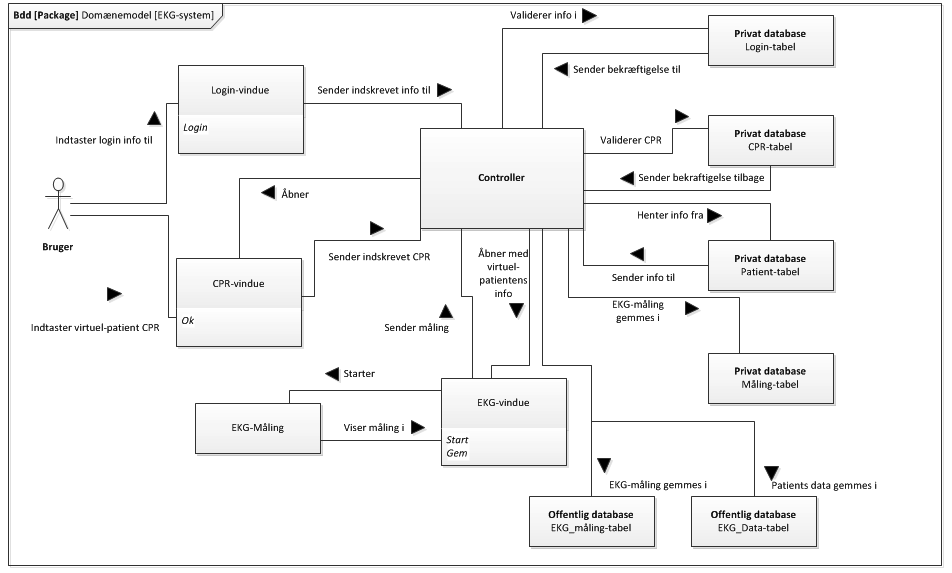
\includegraphics[width=1\textwidth]{Figurer/Snip20150525_18}
	\caption{Domænemodel}
\end{figure}


\subsection{Design}
Alle tanker omkring, hvordan koden skulle være bygget op bunder i trelagsmodellen. Der er derfor sørget for, at der ikke er noget kode, som kommunikerer med et lag, som koden ikke har tilladelse til. Der kan læses mere om trelagsmodellen i dokumentationen 3.3.\\ \\
I dette projekt har der i slutfasen været fokuseret meget på brugervenlighed og feedback til brugeren. Tideligt i projektet var det ikke tydeligt, hvornår der blev foretaget en måling. Dette er blevet tydeliggjort, ved at musen bliver til en cirkel i bevægelse, alt imens der foretages en måling. Der er også lavet et pop-up vindue, som bekræfter, at en måling er blevet gemt.\\ \\
Der er desuden lavet en feature, som viser grid-lines på grafen. I gruppen blev der besluttet, at der skulle være to typer af grids. En lille og en stor type.  De store grids, repræsenterer hver 0,2 sekunder, og de små svarer til 0,04 sekunder. Disse intervaller er fastlagt ud fra standarder for professionelle EKG-displays.  Dette blev herefter implementeret i koden.\\ \\
En anden ting, som har været meget dominerende i overvejelserne, er sikkerhed. Da det er personfølsomme oplysninger, som skal detekteres i dette program, er det vigtigt, at det ikke er alle og enhver, som kan få adgang til oplysningerne. Derfor er der et vindue, som beder brugeren om at logge ind, med et gyldigt brugernavn og kodeord. Login-funktionen validerer, i databasen,  om denne bruger har rettigheder til at få adgang til systemet.\\ \\
Yderligere er der lavet et patient identifikationsvindue, hvor der skal indtastes et CPR-nummer. Dette CPR-nummer er koblet op til en patient, hvis oplysningen ligger lagret i den private database. Når CPR-nummeret indtastes og EKG-vinduet fremkommer, har programmet været nede i den private database og hentet patientens navn, der stemmer overens med CPR-nummeret. Dette gør det muligt, at få udskrevet navnet i EKG-vinduet. Se eventuelt figur 3.5 i dokumentationen.   

\subsection{Implementering}
Analysen er det essentielle i implementeringen. Hvis ikke der er en analyse, der fungerer, så lever programmet ikke op til de stillede krav.\\
Analysen er bygget op omkring tre for-løkker, som identificerer forhøjede amplituder inden for et specielt frekvensspektrum. Ved hjælp af matematikbiblioteket alglibnet2, bliver signalet først konverteret til et komplekst og Furier-transformeret array, som indeholder koordinater som repræsenter vektorer. Vektorernes længde udgør amplituderne i signalet. Denne konvertering, ses på figur 6.4. 

\begin{figure}[H]
	\centering
	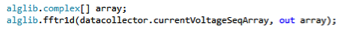
\includegraphics[width=0.8\textwidth]{Figurer/Snip20150525_41}
	\caption{Kode udsnit af analyse implementering}
\end{figure}

Herefter bliver amplituderne regnet ud, ved hjælp af standard formelen for vektorudregning. Disse værdier bliver tilføjet til en ny liste. Dette ses på figur 6.5 nedefor.

\begin{figure}[H]
	\centering
	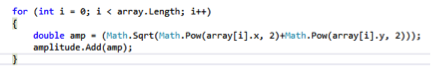
\includegraphics[width=1\textwidth]{Figurer/Snip20150525_43}
	\caption{Kode udsnit af analyse implementering}
\end{figure}

Efterfølgende bliver arrayet udspecificeret til kun, at indeholde de pladser, som repræsenterer amplituderne for det valgte frekvensspektrum. Se figur 6.6 for dette udsnit af koden.  

\begin{figure}[H]
	\centering
	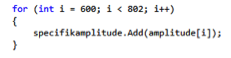
\includegraphics[width=0.6\textwidth]{Figurer/Snip20150525_44}
	\caption{Kode udsnit af analyse implementering}
\end{figure}

Disse værdier bliver derefter tjekket for, om de indeholder en amplitude, som ligger over tærskelværdien. Hvis dette er tilfældet, returnerer metoden ’true’, hvilket repræsenterer, at det er rigtigt, at denne patienten kan have atrieflimren. Hvis der ikke findes en værdi, som er højere end tærsklen, returnerer metoden ’false’, hvilket repræsenterer, at patienten ikke har atrieflimren. Dette kan ses på figur 6.7. 

\begin{figure}[H]
	\centering
	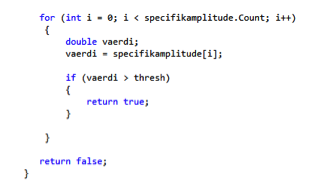
\includegraphics[width=0.8\textwidth]{Figurer/Snip20150525_47}
	\caption{Kode udsnit af analyse implementering}
\end{figure}

Tærskelværdien er blev fundet ud fra testprogrammet, som der kan læses yderligere om i dokumentationen 3.4.3. Tærskelværdien er vurderet, i dette tilfælde, til at være 5,6 V. Der kan desuden også læses yderligere specifikation omkring implementeringen i dokumentationen 3.4. 


\subsection{Test}
I dette projekt er der hverken lavet modul eller integrationstest. I stedet er koden blevet testet efterhånden, som metoder er blevet færdiggjort. Det er også på denne måde, at gruppen har kunnet tjekke, at metoderne ikke melder fejl, eller får systemet til at bryde sammen. \\ \\
Metoden "KørEKG"\  kan give et eksempel på hvordan forløbet har været. "KørEKG"\  er en essentiel del af koden, og det var derfor vigtigt, at den fungerede fra starten af. Her blev den estimerede kode først skrevet, og derefter blev der kørt et EKG for at se, om grafen kom frem. Dette gjorde den ikke i første omgang, og der blev derfor tilføjet en linje kode, som henter den maksimale spænding, som kommer igennem Analog-discovery, og det blev derefter en succes. 

\section{Resultater og diskussion}
Kravene til dette projekt er at afbilde, analysere og gemme EKG-signaler fra virtuelle patienter. Alt dette er lykkes. \\ 
Før det er muligt at starte en måling, skal man igennem et Login-vindue samt et CPR-vindue, hvor man indtaster den virtuelle patients CPR-nummer. Når login og CPR-nummeret er blevet godkendt vises EKG-vinduet, som er vinduet, hvor programmet køres fra. \\ \\
Ved tryk på "Start ny måling"\  går der x-antal sekunder og EKG-signalet bliver afbildet som en graf. Se figur 6.8. 

\begin{figure}[H]
	\centering
	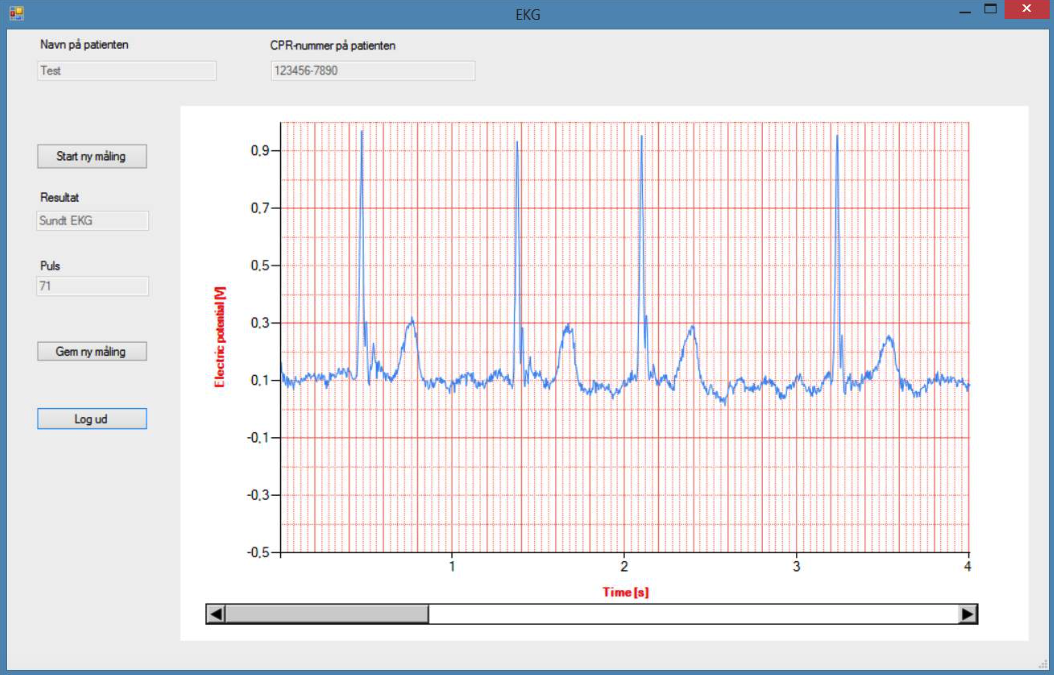
\includegraphics[width=1\textwidth]{Figurer/Snip20150525_25}
	\caption{Visning af EKG-signal samt analyse af sundt EKG-signal}
\end{figure}

Når EKG-grafen vises i EKG-vinduet har programmet også analyseret EKG-signalet i forhold til atrieflimren. Hvis EKG-signalet er normalt skriver programmet "Sundt EKG"\  under Resultat, se figur 6.8. Hvis EKG-signalet afviger fra standardværdierne (se under 3.2) skriver programmet "Tjek for Atrieflimmer!!", se figur 6.9. 

\begin{figure}[H]
	\centering
	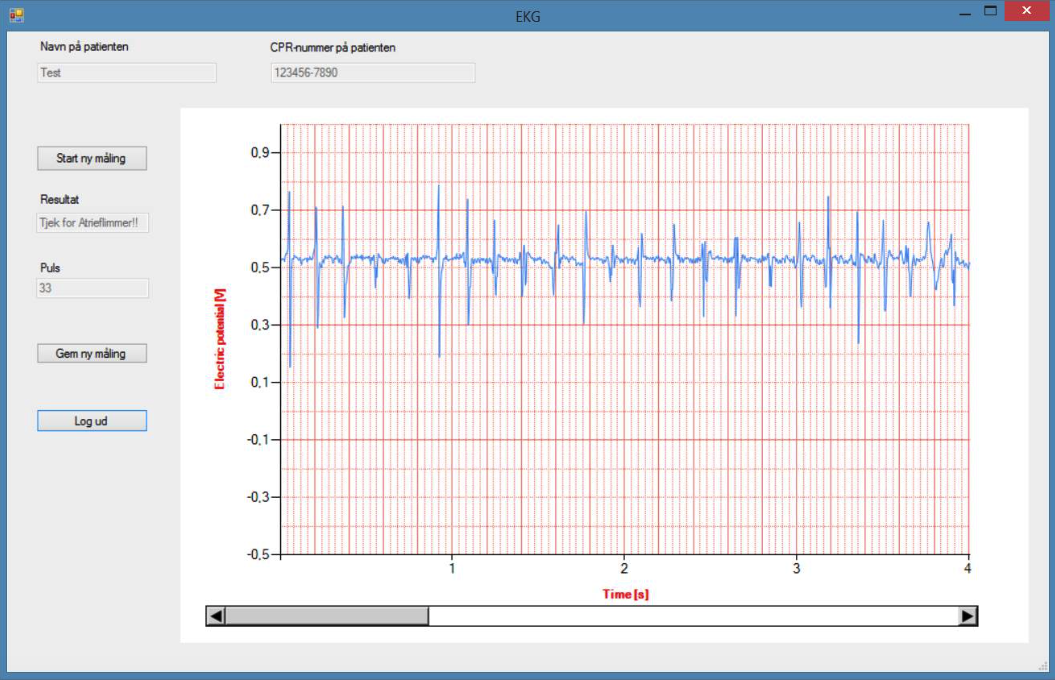
\includegraphics[width=1\textwidth]{Figurer/Snip20150525_26}
	\caption{Analyse af sygt EKG-signal}
\end{figure}

Efter visningen samt analysen af EKG-signalet skal målingens data gemmes i en privat- og offentlig database. Dette sker ved tryk på "Gem ny måling", hvorefter et pop-up vindue fremkommer og bekræfter handlingen. Efterfølgende kan man i den private database under "Måling"\--tabellen, se de gemte målinger, se figur 6.10.   

\begin{figure}[H]
	\centering
	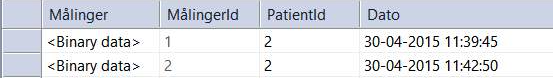
\includegraphics[width=1\textwidth]{Figurer/Snip20150525_27}	
	\caption{Lagring af data i privat database}
\end{figure}

I den offentlige database er der to tabeller. Den ene hedder EKG\_Data, hvor den virtuelle patients og brugerens data gemmes, se figur 6.11. Den anden hedder EKG\_måling, hvor informationer omkring selve målingen gemmes, se figur 6.12. 

\begin{figure}[H]
	\centering
	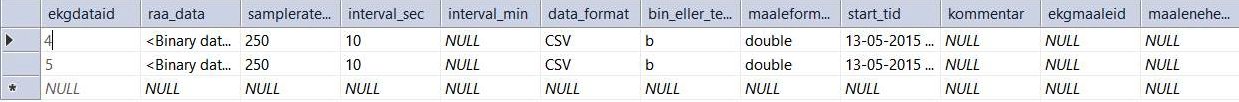
\includegraphics[width=1\textwidth]{Figurer/Snip20150525_28}
	\caption{Lagring af den virtuelle patients- og brugerens data i den offentlig database}
\end{figure}

\begin{figure}[H]
	\centering
	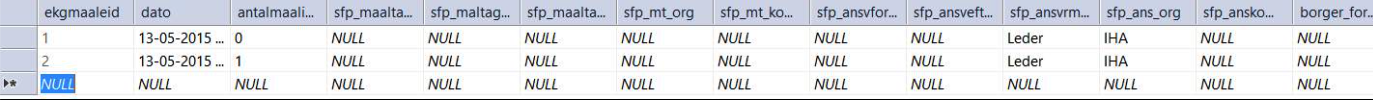
\includegraphics[width=1\textwidth]{Figurer/Snip20150525_29}
	\caption{Lagring af målingens data i offentlig database}
\end{figure}

Med hensyn til visningen af målingen, kunne der godt have været et mere præcist gitter, således at brugeren nemmere kunne aflæse ud fra grafen om patienten har atrieflimren. Det kan godt lade sig gøre at aflæse på nuværende tidspunkt, men det er mindre præcist, da ternene ikke er kvadratiske.

Det har ikke været muligt at gøre analysen så præcis, at den kunne detektere atrieflimren helt præcist, men derimod gør den brugeren opmærksom på, at der er en anormalitet i forhold til et normalt EKG-signal. Analysen kunne ikke gøres præcis, da der findes mange forskellige typer af EKG-signaler, der repræsenterer atrieflimren, som følge af, at mennesker er forskellige.

Da det kom sent ud, at der skulle kunne gemmes i en offentlig database, er flere af værdierne blev fravalgt. Dog kunne der have været indskrevet nogle flere værdier, således at f.eks. patientens CPR-nummer og navn kunne lægges ind og gemmes i tabellen EKG\_Data.

I kapitel 4 i dokumentationen kan resultatet af accepttesten læses.

Projektet har krævet, at det har været nødvendigt at opsøge viden ud over pensum. Eksempelvis er der brugt BLOB, som er benyttet til gemme-funktionen i den private- og offentlige database. Ydermere er der brugt et matematikbibliotek, alglibnet2, til udarbejdelse af analyse.

\section{Opnåede erfaringer}
Gruppen har opnået stor erfaring i forhold til at koble fagene sammen, dette gælder i særhed programmering og ISE. Arbejde med metoderne fra fagene, har givet erfaringer i til at bruge teorien i praksis. Desuden har der været stor fokus på udarbejdelse og opbygning af rapport samt dokumentation og de tilhørende logbog og mødereferater. 

\textbf{Lise Skytte Brodersen}\\

\textbf{Mads Fryland Jørgensen}\\

\textbf{Albert Jakob Fredshavn}\\
I dette projektet har jeg arbejdet med projektdokumentationen. Til at arbejde med dette har vores del af projektgruppen benyttet de redskaber som blev undervist i, i ISE lektionerne, samt dele af vores anatomi og fysiologi undervisning. De modeller og metoder som blev taget i brug var meget overensstemmende med det som vi havde lært og gav en god relation til det arbejde vi skulle igennem. Vi blev delt i to undergrupper gennem projekt, en der stod for programmeringen og en der stod for dokumentationen gennem projektet. Denne opdeling og uddelegering gjorde at den ene gruppe ikke havde særlig stor indflydelse på hvad den anden gruppe lavede, i henhold til at følge processen gennem projektet. Det er dog blevet gennemgået ned til detaljer og beskrevet i selve kode-delen af programmet med udkommenterede linjer tekst. \\
Projektarbejdet i gruppen har forgået ganske godt. Der blev fra start til slut holdt regelmæssige gruppermøder med vores projektvejleder. Dette har klart været en fordel da det har forventningsafstemt vores forskellige opgaver gennem projektet. Samtidig har gruppen, i nogen omfang, været god til at kommunikerer med hensyn til hvor langt de enkelte var, og med hvad. Stemningen i gruppen har været ambitiøs uden at man følte et tungt pres på skuldrene. Ligeledes har stemningen været afslappet nok til at man kunne stille spørgsmål og få hjælp til diverse opgaver igennem projektets forløb.\\

\textbf{Malene Cecilie Mikkelsen}\\
Da vi startede projektet, delte vi gruppen op i to grupper, hvilket vi følte var en nødvendighed for at kunne nå det hele. Desværre havde det den følgevirkning, at kommunikationen mellem de to grupper blev lidt halvhjertet, således at der af flere omgange blev brug for at lave ændringer, og der var nogle enkelte diskussioner mellem grupperne. I gruppen var det aftalt ikke at have en leder, men jeg synes ikke, at det fungerer ordentlig, da der mangler en, som har noget overblik. Heldigvis tog Lise styringen i løbet af projektet, dog havde det været en fordel, hvis dette havde været klart fra starten. 
Selve emnet har været meget relevant, og det har givet en del erfaring til arbejdsmarkedet. Særligt den ekstra del med den ekstra database, som kom ud, da vi efterhånden troede, at vi var færdig, pressede gruppen en del, men gav en erfaring med, at det er sådan noget, som man kan komme ud for senere på arbejdsmarkedet.
Projektet er blevet fuldført, men jeg synes, at vi kun lige har fuldført den. Vi havde mange gode ideer, da vi startede, men det mundede ud i, at vi kun fik lavede det mest nødvendige. Til næste projekt kunne jeg godt tænke mig, da der blev arbejdet lidt mere fokuseret, og at der blev stillet lidt højere krav indenfor gruppen.

\textbf{Mohammed Hussein Mohamed}\\
Det er lykkes at udvikle et software produkt, der kan afbillede, detektere atrieflimren samt gemme et EKG-signal i en privat database oprette af gruppen og i en offentlig database, som er udleveret af vejlederen. Som forventet bliver der brugt en del tid på, hvordan designet til softwaren skulle se ud og hvad for nogen use cases, som er relevant at have med. Ambitionerne var høje og ideerne fejlede ikke noget i starten, men undervejs under projektet har vi droppet et par funktioner som vores software burde have, da vi ikke kunne opfylde det pga. vores begrænsede viden på området.

Vi har delt os i to større grupper som hver havde deres ansvarsområde. Den ene gruppe designede og programmerede og den anden gruppe lavede system og use case beskrivelse arkitektur. Jeg var en del af den gruppe, der programmerede. Derfor var det mest af det jeg har været med og ikke så meget til rapportskrivning. Stemning i gruppen har været fint og jeg har oplevet at alle har bidraget med det de kunne.

Den tværfaglige viden i dette semesterprojekt er ifølge mig kommet til udtryk. Det vi har lært i de forskellige fag kunne direkte anvendes sammenlignet med sidste semesterprojekt, hvor den tværfaglig ikke var så tydelig. Dette har efter min mening været interessant. Jeg var især begejstret for faget ISE og hvordan faget havde så meget relevans i semesterprojektet.

Måden vi har arbejdet med dette projekt kunne ligne, hvordan man arbejder ud i den virkelige verden, altså at kunne udvikle et produkt i samarbejde med en kunde, hvor kunden og udvikleren af produktet stiller krav til produktet. Undervejs kan kunden ændre krav og udvikleren må herefter indstille sig på disse nye krav. Dette scenarie blev vi testet i på dette semesterprojekt. Vejlederen har i slutningsfasen af semesterprojektet ændret lidt på kravene, hvor vi fik udleveret en offentlige database som vores målinger og data skulle gemmes.  Heldigvis krævede det ikke megen kode og tid, men gruppen var ikke begejstret for den sene udmelding fra vejlederen uden at flytte deadline for projektets færdiggørelse.

Overordnet set har dette projekt været fint og lærerigt. 

\textbf{Sara-Sofie Staub Kirkeby}\\
I dette projekt, har jeg primært arbejdet med det programmeringsmæssige aspekt. Personligt, syntes jeg det har været en anelse frustrerende, da der i den sammenhæng, er dukket nogen ting op, som ikke har været en del af vores undervisning, i dette semester. Det har krævet meget tænkning ud af boksen. Dette har selvfølgeligt også gjort, at vi har været tvunget til, at lære os selv, yderligere ting. \\
Jeg har siddet med det overordnede ansvar for analysen, og det viste sig at være mere problematisk, end først regnet. Analysen blev ændret tre gange undervejs, og hver eneste gang, har der været behov for, at skrive analysen fuldstændig om. Her har vejleder dog været rigtigt god til, at træde til, og give et andet syn på, hvordan analysen kunne laves, og det hjalp meget.\\ 
Et andet problem har været, at vi valgte at dele gruppen op i to; en der lavede det meste tekstarbejde, og en anden del, som stod for programmeringen. Kommunikationen imellem de to undergrupper, har til tider ikke været særligt godt, og det har betydet at vi er blevet nødt til at ændre nogen ting undervejs. \\
Jeg mener generelt at jeg har lagt et godt stykke arbejde i gruppen, og jeg har forsøgt at gøre så meget jeg overhovedet kunne. Jeg har lært meget om EKG-signaler og deres karakteristikker, samt omkring, hvordan sådan et program skal programmeres. Jeg kunne dog eventuelt godt have forsøgt at tage mere initiativ, og have taget lidt mere kontakt med skriveholdet. \\
Projektet er efter min mening gået rigtigt godt, og jeg mener at det er et stykke arbejde vi godt kan være stolte af.

\textbf{Martin Banasik}\\
I dette 2. semesterprojekt som omhandler måling af EKG, har jeg været med til at programmere vores program fra start til slut. Dette har omfattet vores første overvejelser hvordan vores program skulle se ud og hvilke funktioner det skulle have, til et færdig program som jeg er godt tilfreds med. I forprojektet fandt jeg det svært at komme i gang med og forstå hvad det skulle kunne, men efterhånden jeg man satte sig mere ind i koden, hjalp det på forståelsen og kunne gøre brug af og overføre de ting jeg havde lært i programmering til vores eget projekt og program. Det har øget min interesse for programmering og finder det spændende at lave et program fra bunden, ud fra fordefineret krav og funktion. 

Jeg synes at samarbejdet har været fint og har fungeret i programmerings gruppen. Selvom at vi i starten var i tvivl om hvordan vi skulle gribe det hele an og samtidigt med at vi alle havde vores egne ideer til hvordan det skulle være, synes jeg at vi er kommet frem til et resultat, hvor alle har haft deres indflydelse. Der var ideer som vi gerne ville have med i programmet, men efter evne og deadlines blev droppet, hvilket man kunne til en anden gang have mere fokus på, så disse blev en realitet. 

\textbf{Cecilie Ammitzbøll Aarøe}\\
Igennem dette projekt arbejdede jeg i den gruppe som bla. udarbejdede projektdokumentationen. Det gjorde at jeg fik mulighed for at arbejde med nogle af de værktøjer, som vi har lært i ISE. En ulempe har dog været, at jeg dermed ikke var med til at programmere programmet. Den del af gruppen, som programmerede, var dog meget gode til at udkommantere programmering, så vi andre nemt kunne sætte os ind i den. Desuden afholdte vi enkelte møde, hvor programmeringen blev gennemgået i de mindste detaljer. Men det er stadigvæk ikke det samme som at sidde med det selv.\\
Jeg synes gruppen har arbejdet godt sammen, og vi havde fra starten afstemt vores forventninger til projektet. At disse forventninger så var lidt højere end det var muligt at efterkomme, er noget der altid vil ske i starten af et projekt. Men jeg vil hellere hav store forventninger til et projekt og så afstemme dem med hvad der er realistisk, frem for at sætte baren lavt fra starten.\\
Vi havde også lidt kommunikations vanskeligheder i starten af projektet. Dokumentationsgruppen skulle designe systemet udfra funktionelle og ikke-funktionelle krav. Vi rådførte os med programmeringsgruppen, men der opstod en misforståelse mellem grupperne, som gjorde at vi ikke helt havde forstået hvad systemet helt præcist gjorde.\\
Men alt i alt synes jeg, det har været en god oplevelse at lave dette projekt. Gruppen har fungeret rigtig godt. Der har været en god stemning, og vi har været gode til at hjælpe hinanden, når der var brug for det.

\section{Fremtidigt arbejde}
Som følge af at projektet er tiltænkt som en prototype, er der løbende gennem projektudførelsen opstået en masse muligheder og idéer for videreudvikling af systemet. \\\\
Den første helt basale idé, som også er forsøgt udført sideløbende i projektet, er etablering af en "opret ny patient"\--funktion. Funktionen skal muliggøre, at brugeren kan oprette en ny patient i systemet i forbindelse med indtastning af patientens CPR-nummer. Funktionen skal fungere således, at hvis ikke det indtastede CPR-nummer i forvejen er kendt i systemet, skal skridtet efter CPR-vinduet være et nyt "Opret Patient"\--vindue. Her skal brugeren kunne indtaste relevante oplysninger omkring patienten, og til slut oprette patienten i både den private- og offentlige database.\\\\
Et ideelt område til videreudvikling er brugervenlighed, både på software plan og i særhed på hardware plan.\\
Software kan udvikles i en retning, hvor det bliver lettere og mere overskueligt for brugeren, at analysere og evaluere EKG-signalet. En forbedring ville være, at der skal være mulighed for at trække en eller flere x- og y-cursors ned over EKG-signalet, og dermed få vist amplitude, tid og relevante intervaller. Herefter kunne en mulighed være, at de observerede værdier kunne gemmes som tilhørende tekst til det specifikke EKG-signal. \\
Sideløbende, imens EKG-målingen foretages, vil det være muligt, at have direkte adgang til den pågældende patients sygejournal. Adgangen til sygejournalen skal kunne læses i et andet vindue, som er synligt samtidig med EKG-vinduet arbejder, hvorefter det er muligt at skifte mellem disse vinduer, og tilføje ændringer, notater etc. i journalen. Med andre ord skal systemet understøtte den elektroniske patient journal.\\ \\
Den endelige udgave af softwaren skal implementeres på et mere brugervenligt interface, eksempelvis en tablet eller lignende. Samtidig kan systemet være tilknyttet en håndholdt EKG-måler, i form af en holter, hvorefter softwaren aflæser data, og udskriver på tabletten.\\ Desuden skal det være muligt for brugeren at vælge indstillinger alt efter, hvad der ønskes analyseres for. Prototypen er kun tilpasset analyse for atrieflimren, men med det endelige produkt skal være muligt at kunne vælge undersøgelse for eksempelvis andre hjertesygdomme. De forskellige undersøgelser skal derudover også kunne mixes på kryds og tværs, hvis patienten har blandede symptomer, således at der søges for flere sygdomme. Dette vil medføre, at brugeren kan tage udstyr med sig på hjemmebesøg, såvel som at patienten selv kan foretage en måling.


\chapter{Konklusion}
I dette projekt, er der blevet udviklet en software prototype, som kan afbillede og analysere EKG-signaler. 
Gruppen startede ud med høje ambitioner, omkring prototypen, men opdagede hurtigt, at tankerne omkring hvordan prototypen ideelt skulle være, og hvad der reelt kunne udvikles, ikke stemmede overens. 
På trods af de høje forventninger, har gruppen formået at opfylde alle overordnede krav, som blev sat i starten af projektet. Dette kan ses på den gennemførte accepttest, som kun havde en designrelateret afvigelse. Kravene om at afbillede og analysere et EKG-signal er blevet opfyldt, og det er også lykkedes gruppen at implementere, at gemme i en privat database. 
Gruppen har oplevet at, det har været en udfordring, at udvikle en analyse, som kunne dække over varierende signaler. Det blev klart, at et EKG-signal diagnosticeret med atrieflimren, kan variere i udseende, og det blev derfor svært for gruppen, at udvikle en algoritme, som kunne dække over flere signaler. Der blev derfor udarbejdet en algoritme, ud fra et specifikt signal. 
Kravet fra Sundhedsstyrelsen, om en offentlig database, blev præsenteret sent i arbejdsprocessen, men det lykkedes gruppen at implementere det, uden store vanskeligheder. 
Udviklingsprocessen har været præget, af at gruppen har tænkt meget over, hvordan dette system ville skulle fungere ude i virkeligheden. Dette kan ses på nogen af de krav, som gruppen selv har sat til projektet. 
Projekt er overordnet set, gået godt, og gruppen er tilfreds, med produktet. 

\begin{thebibliography}{9}
\bibitem{a} Olav Sand m.fl. \& Jan G. Bjålie - \textit{"Menneskets anatomi og fysiologi"}\\ Gads Forlag, 18. August 2008
\bibitem{b} Sanford Friedenthal, Alan Moore og Rick Steiner - \textit{"A Practical Guide to SysML"} \\Morgan Kaufmann OMG Press, 17. Oktober 2011
\bibitem{c} Craig Larman -
	\textit{"Applying UML and Patterns"}\\ Prentice Hall, 30. Oktober 2004
\bibitem{j} Poul Staal Vinje - \textit{"Projektledelse af systemudvikling"}\\ Nyt Teknisk Forlag, 23. April 2004
\bibitem{k} John G. Webster \textit{"Medical Instrumentation - application ad design"}\\ John Wiley & Sons, 4th edision
\bibitem{d} \textit{http://www.si-folkesundhed.dk/upload/hjertekarsygdomme\_i\_2011-2\_rapport.pdf}
\bibitem{e} \textit{https://www.sundhed.dk/borger/sygdomme-a-aa/hjerte-og-blodkar/sygdomme/hjertearytmier/atrieflimren-og-flagren/}
\bibitem{f} \textit{www.physionet.org}
\bibitem{g}\textit{http://www.hjertelunge.dk/hjertesygdomme/hjerte\_og\_kredsloeb/hjertet/}
\bibitem{h} \textit{http://en.wikipedia.org/wiki/QRS\_complex\#/media/File:SinusRhythmLabels.svg}
<<<<<<< Updated upstream
\bibitem{i} \textit{http://www.health.harvard.edu} 
=======
\bibitem{i} \textit{http://www.health.harvard.edu/heart-health/atrial-fibrillation-common-serious-treatable}
>>>>>>> Stashed changes

\end{thebibliography}

\backmatter
\chapter{Bilag}

%\bibliography{bibliografi/PRJ3}    % Sætter bibliografien bagerst i dokumentet. Bruger bib-filen PRJ3.

\end{document}